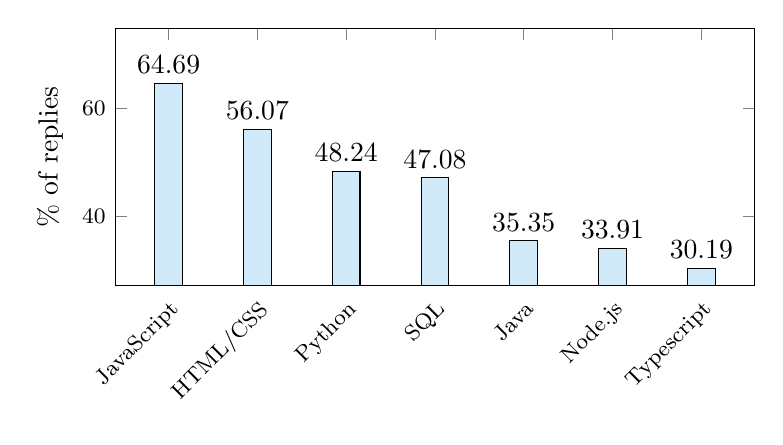
\begin{tikzpicture}
    \definecolor{myblue}{RGB}{13,98,153}
    \definecolor{mybluefill}{RGB}{208,234,250}

    \begin{axis}[
        symbolic x coords={JavaScript, HTML/CSS, Python, SQL, Java, Node.js, Typescript},
        xtick=data,
        width=0.8\textwidth,
        height=0.4\textwidth,
        x tick label style={rotate=45, font=\footnotesize, anchor=north east}, 
        y tick label style={font=\footnotesize}, 
        ylabel = {\% of replies},
        nodes near coords,
        ymin=27, ymax=75
    ]
        \addplot[ybar,black,fill=mybluefill] coordinates {
            (JavaScript, 64.69)
            (HTML/CSS, 56.07)
            (Python, 48.24)
            (SQL, 47.08)
            (Java, 35.35)
            (Node.js, 33.91)
            (Typescript, 30.19)
        };
    \end{axis}
\end{tikzpicture}
